\section{Brown Dwarf vs Giant Planet}
\label{sec:BDvsGP}
\subsection{Hot Star vs Cold Star}
\label{sec:hot_vs_cold}
\cite{Marley2007} suggested that young giant planets formed by core accretion in a protoplanetary disk should
have a much lower entropy content at young ages than objects of same mass and age formed by gravitational collapse, 
either from a pre-stellar core or by disk instability.
Consequently, the first type of objects should be significantly smaller, cooler and (about 100 times) fainter at young
ages than the second ones. This gave rise to the so-called ?cold start? observational signature, characteristic of young
giant planets formed by core accretion, vs the ?hot start? one, typical of young objects, GP?s or BD?s, formed by collapse
to distinguish these objects from their distinct formation mechanisms. 

This suggestion, however, directly relies on two assumptions. 
First of all, the assumption that GP?s formed by core accretion have a low entropy content implies 
that all the energy of the accretion shock through which most of the planetary mass is processed is radiated
away, leaving the internal energy content of the nascent planet unaffected. This is characteristic of a so-called 
supercritical shock. In that case the radiative losses at the accretion shock act as a sink of entropy. This assumption,
however, has never been verified. In fact, a proper treatment of the accretion shock at the onset of a pre-stellar core 
formation, the so-called second Larson?s core, shows that the shock in that case is sub-critical, with essentially all the 
energy from the infalling material been absorbed by the stellar embryo \citep{Vaytet2013, Tomida2013, Bate2014}. 
Although the two formation conditions differ in several ways, they share enough common processes to
at least question the assumption of a supercritical shock for planet formation. 
The second underlying assumption about this scenario is the assumption that BD?s form with a high entropy content. 
Again, such an assumption is not necessarily correct. Initial conditions for brown dwarf formation are rather uncertain. 
Figure \ref{fig:evolution} (see also \cite{Mordasini2012a, Mordasini2013, Spiegel2012}) compares the early 
evolution of the luminosity for a 5 $M_{Jup}$ object under several assumptions. 
The blue solid and dot-dash lines represent giant planet early evolution. 
assuming that either 
the accretion energy is entirely converted to radiation, i.e. a supercritical 
shock condition as in \cite{Marley2007}, or that this energy is absorbed by the planet, i.e. a sub-critical shock
with no radiative loss at the shock. 
The former case yields a low entropy content thus a low luminosity at the end of
the accretion shock while in the second case the luminosity slowly decreases from its value at the end of the shock,
two orders of magnitude brighter, for several Myr?s. The red long-dash and short-dash lines correspond to the early
evolution of a brown dwarf \citep{Baraffe2003} assuming an initial radius $R_i \sim 8 R_{Jup} (\simeq 0.8 R_{Jup})$ (short-dash) or
$R_i \sim 1.6~ R_{Jup}$ (long dash). This corresponds to specific entropies $\tilde{S?} \simeq 1.1 ? 10^9$ and 
$\simeq 8.0 ? 10^8 erg~ g^{?1} K^{ ?1}$ , respectively.

\begin{figure}[!t]
\vspace{0cm}
\centerline{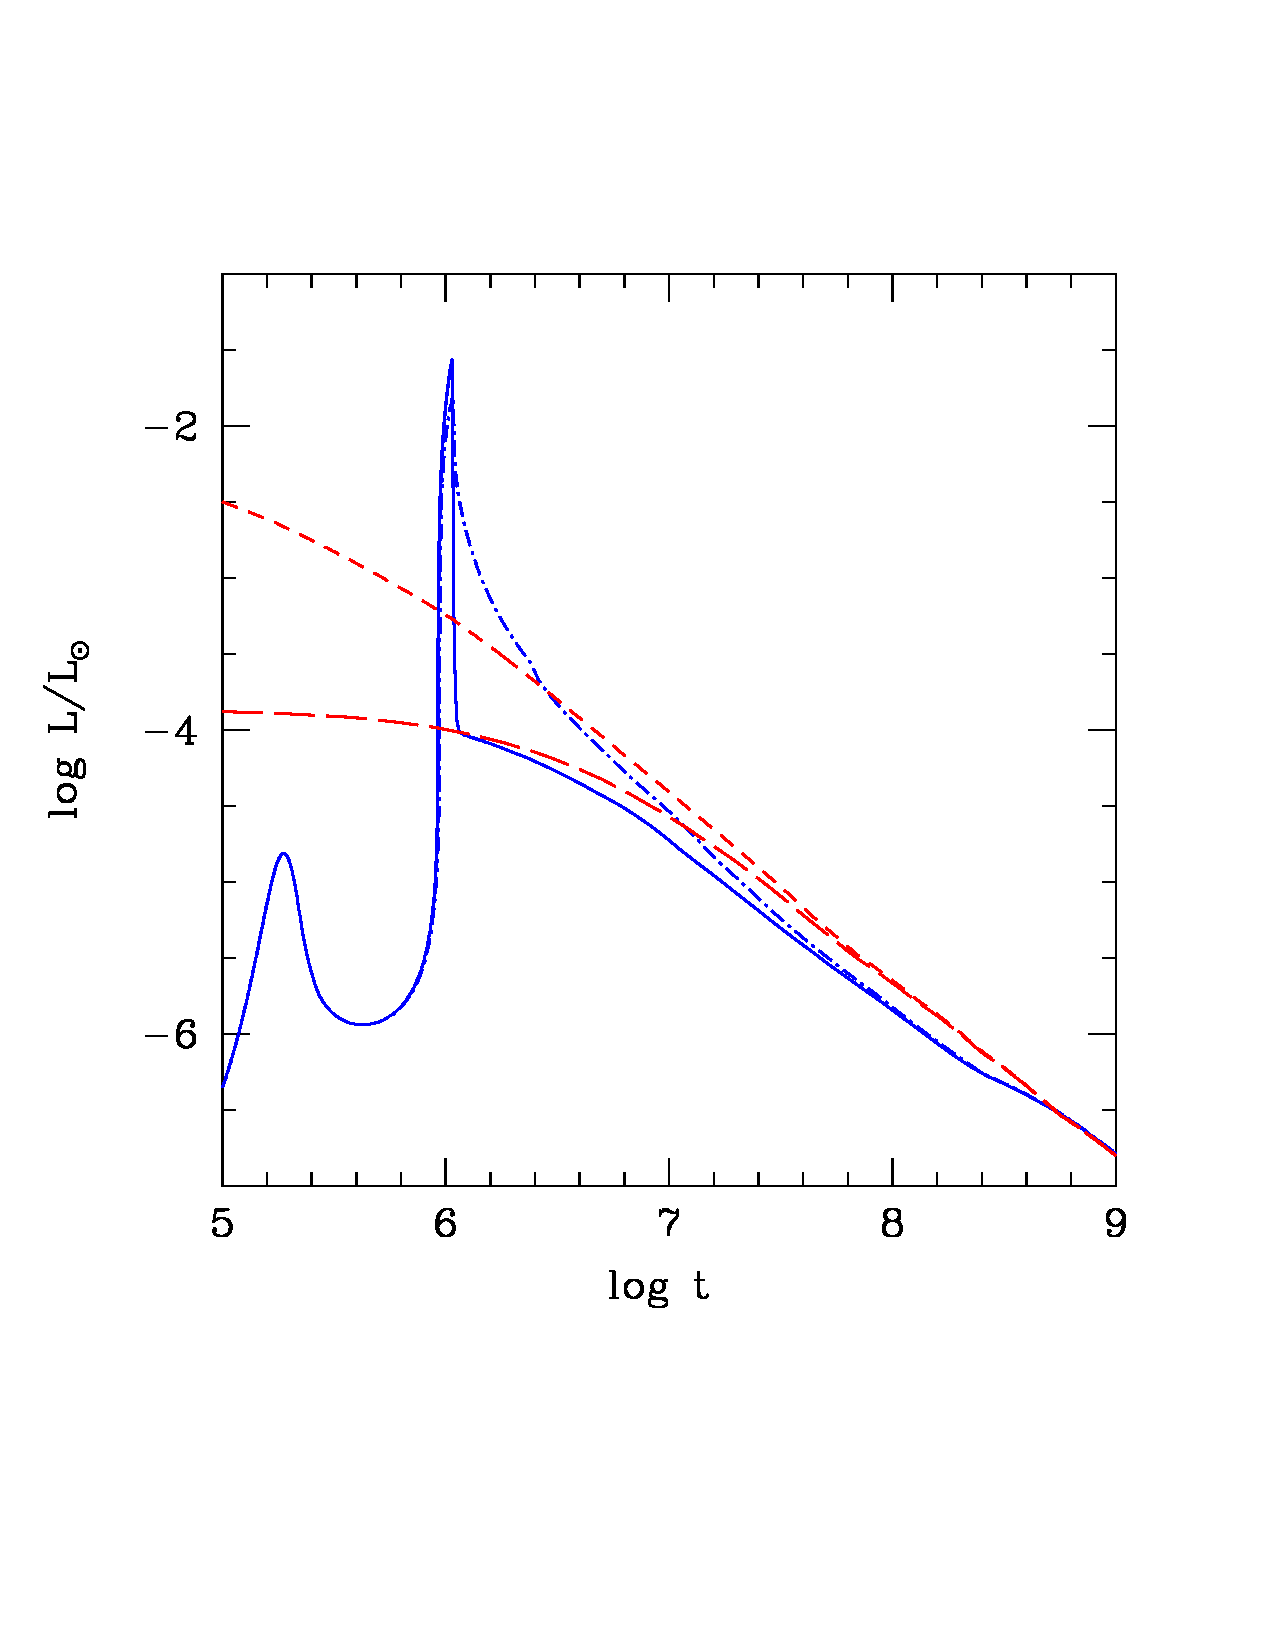
\includegraphics[trim=0.5cm 5.5cm 0.5cm 4.5cm,clip, width=0.6\textwidth]{fig_hot_cold_start_L2.pdf}}
\caption{Early evolution of a 5 Jupiter-mass object according to
different formation scenarios. Blue: object formed by core accretion assuming 
either a supercritical shock (solid line) or a subcritical shock (dash-dot line) 
at the end of the accretion process, after \cite{Mordasini2012a}. 
Red: object formed by gravitational collapse for two arbitrary initial conditions (see text), 
after \cite{Baraffe2003}}
\label{fig:evolution}
\end{figure}


As seen in the figure, depending on the outcome of the accretion shock episode in one case and on the initial 
radius (thus entropy content) in the second case, and given the
long Kelvin-Helmholtz timescale for such low-mass objects (several Myrs) young planets formed by core accretion can
be as bright and even brighter than young BD?s for several Myrs. (Magneto)Radiation-hydrodynamics calculations of
the collapse of prestellar cores \citep{Tomida2013, Vaytet2013} seem to exclude the above rather extreme 
?cold start? initial condition for a proto-BD, even though calculations have not been performed yet for such low masses.
They suggest initial entropy contents and radii closer to the hot-start case, the outer region of the protostellar core been
heated up by the shock and attaining a higher entropy. Hot-start conditions for core-accretion GP?s, probably in between 
the two above extreme cases, however, are presently not excluded. Interestingly enough, measured temperatures
and luminosities of some directly-imaged exoplanets, notably $\beta$ Pic b and $\kappa$ And b, are consistent with hot-start like
conditions and seem, so far, to exclude the coldest range of initial conditions for these objects \citep{Currie2013,
Marleau2013}. Therefore, at least in the absence of a better knowledge of the accretion shock 
condition at the end of the core accretion process, the cold start - hot start argument does not provide a reliable diagnostic
to distinguish core accretion from gravitational instability formed objects. 
For sure there is no one-to-one correspondence between cold start vs. hot
start conditions and core accretion vs disk or core collapse.

\subsection {Deuterium Burning}
The distinction between brown dwarfs and giant planets is a topic of intense debate. 
In 2003, the IAU has adopted the deuterium-burning (DB) minimum mass, $\sim 10~ M_{Jup}$ , as the official distinction between the
two types of objects. 
Deuterium burning has no impact on star formation and a negligible impact on stellar/BD evolution \citep{Chabrier2000c}. 
This is in stark contrast with the lifetime impact of hydrogen-burning, making H-burning a genuine physical mechanism
distinguishing objects in nuclear equilibrium for most of their lifetime, defined as stars, from objects which lack 
significant support against gravitational contraction and keep contracting for ever since their birth, defined as brown dwarfs.
One of the strongest arguments against deuterium burning to distinguish planets from brown dwarfs is
2M 1207 b \citep{Chauvin2005}, which is a $\sim 4~ M_{Jup}$ companion to a $\sim 20~ M_{Jup}$ brown dwarf. Thus, the companion is 
firmly in the non deuterium burning mass regime, but with a system mass ratio of 20\%, the couple appears to be best
described as an extension of the brown dwarf binary population rather than a planetary system. In contrast, it is
presently not excluded that genuine planets formed by core accretion, characterized by a significant heavy element 
enrichment, reach masses above the deuterium burning limit and thus ignite D-burning in their core \citep{Baraffe2008, Molliere2012, Bodenheimer2013}.

\subsection {The Brown Dwarf/Planet Overlapping Mass Regime}
There is now ample evidence for the existence of free floating brown dwarfs with
masses of the order of a few Jupiter masses in (low extinction) young clusters and in the field, see \cite[e.g.][]{Caballero2007}, 
with a mass distribution consistent with the extension of the stellar IMF into the BD regime. The brown
dwarf and planet mass domains thus clearly overlap, arguing against a clear mass separation. The fundamentally
different mass distribution of exoplanets detected by radial velocity surveys, with the mass function rising below
$\sim 30~ M_{Jup}$ \citep{Mayor2011}, in stark contrast with the BD mass distribution clearly suggests two 
distinct populations, with different origins.
Of particularly noticeable interest at this stage are the transiting objects Hat-P-2b, with a mass of $9~ M_{Jup}$ 
(Bakos et al., 2007b) and Hat-P-20b, with a mass of $7.2 M_{Jup}$ \citep{Bakos2011}. Both objects are too dense to be brown
dwarfs. Assuming that the observational error bars on the radius are reliable, and given the age inferred for theses 
system, the observed mass-radius determinations imply significant enrichment in heavy material, revealing their planetary
nature \citep{Leconte2009, Leconte2011}. This shows that planets at least 9 times more massive than Jupiter, close to the
DB limit, can form according to the core-accretion scenario, possibly from the merging of lower mass planet embryos.
Note that while massive objects like HAT-P-20 b approach the upper limit of the mass distribution predicted by the core
accretion scenario \citep{Mordasini2012b}, its large metal enrichment ($M_Z \sim 340 M_{\oplus}$, \cite{Leconte2011}) 
certainly excludes formation by gravitational collapse.
According to the arguments given above, the present IAU definition, based on a
clear-cut mass limit between BD?s and planets, is clearly incorrect and confusing and should be abandoned.

\section {Conclusion}
Even though it is probably still premature to reach definitive conclusions about brown dwarf and giant planet formation 
and we must remain open to all possibilities, the confrontation of the various theories with observational constraints 
suggests some reasonably sound conclusions. The ability of BD?s to form in isolation
and in wide binaries; the similarity of BD number-density in low and high-density environments, indicating
no significant dependence of BD abundances upon stellar density; the emerging observations of isolated proto-BD?s
and pre-BD cores; the many observational properties shared by young BD?s and young stars; the observed close 
similarity between the pre-stellar/BD core mass function and the final stellar/BD initial mass function; 
the BD IMF been consistent with the natural extension of the same stellar IMF down to the nearly bottom of the BD domain. 
All these points provide evidence that dynamical interactions and dense cluster environments, disk fragmentation or photoionizing 
radiation are not required for BD formation. In contrast, all these properties are consistent with BD formation being a
natural scaled down version of star formation by the turbulence induced fragmentation of molecular clumps, leading
to the formation of pre-stellar and pre-BD cores. It is not excluded, however, that, under some specific circumstances
(very dense environment, very massive disks), the other aforementioned mechanisms might play some role but, in
the absence of clear observational evidence for this so far, they seem unlikely to be the dominant mechanisms for star
and BD formation.
Conversely, the overwhelming majority of planet discoveries are consistent with planet formation by core accretion.
As examined in section 5.3, this scenario might also explain planet formation at large orbital distances, not mentioning
the possibility to explain such objects by planet scattering or outward migration. Here again, alternative scenarios like
disk fragmentation might occur in some places, notably in massive circumbinary disks, and thus explain some fraction of the planet population (possibly $\sim$ 10\% or so, \cite[e.g.][]{Vorobyov2013}), but they can hardly be considered as
dominant scenarios for planet formation. Hybrid scenarios invoking both gravitational fragmentation at large orbital
distances followed by inward migration, invoking even in some cases evaporation seem
to raise even more problems than they bring solutions, as migration can only exacerbate problems with the gravitational 
instability. Not only one needs to form planets by GI but one needs to prevent them to migrate rapidly all the way
into the star (Vorobyov and Basu, 2006b; Machida et al.,2011; Baruteau et al., 2011; Vorobyov, 2013). Migration,
however, is very likely and fast given that, in that case, the disk mass must be very high, a requirement for GI to occur. 
If planets indeed form this way, this requires very finetuning conditions, making the branching ratio for this route
very small.

Finally, as discussed in ?\ref{sec:BDvsGP}, there is ample evidence that the planet and brown dwarf domains overlap and that deuterium 
burning plays no particular role in the formation process. There is now growing evidence, possibly including the
WISE survey for the field population, for the existence of non-deuterium burning free floating brown dwarfs
and, conversely, no physical arguments against the possibility for genuine planets to ignite D-burning in their core.
This again shows that the IAU definition has no scientific justification and only brings scientific and mediatic 
confusion. This also argues against the use of specific appellations for free-floating objects below the D-burning limit, these
latter being simply non D-burning brown dwarfs.

Given the arguments examined along this review, it seems rather secure to argue that BD?s and GP?s represent 
two distinct populations of astrophysical bodies which arise dominantly from two different formation mechanisms.
While BD?s appear to form preferentially like stars, from the gravoturbulent fragmentation of a parent (possibly 
filamentary) molecular clump, GP?s arguably form essentially by core accretion in a protoplanetary disk, i.e. from the
growth of solids (planetesimals, pebbles) yielding eventually the accretion of a surrounding gas rich H/He envelope.
So, the very definition of a brown dwarf or a giant planet is intrinsically, tightly linked to its formation mechanism.
%As briefly discussed below and in ?3.2, this latter should leave imprints which might be observationally detectable.
As examined in ?\ref{sec:hot_vs_cold}, the luminosity or effective temperature at early ages, however, cannot be used as a diagnostic
to distinguish between these two populations. On the other hand, we argue in this review that planets are necessarily
companions of a central, significantly more massive object. 
Consequently, free floating objects down to a few $M_{Jup}$ can rather unambiguously be identified as genuine (non D-burning) brown dwarfs, 
and one should stop giving them different names, which simply adds to the confusion. 
This is the most direct observational distinction between
the two types of objects. Ejected planets probably exist and weaken this statement but they are unlikely to represent
a significant fraction of the population. The diagnostic is less clear for wide companions to stars, except if the mass
ratio can safely exclude one of the two possibilities. According to the distinct formation scenarios, planets should
have a substantial enrichment in heavy elements compared with their parent star, as observed for our own solar giant
planets, whereas BD?s of the same mass should have the same composition as their parent cloud. As suggested in
\cite{Chabrier2007} and \citep{Fortney2008}, giant planets should bear the signature of
this enhanced metallicity in their atmosphere. Spectroscopy or even photometry of atmospheric chemical abundances,
notably metal-dominated compounds like e.g. $CO$ or $CO_2$ may provide clues about the formation mechanism and thus
help identifying the nature of the object. In the absence (so far) of clear observational diagnostics (mean density, 
atmospheric abundances, oblateness, etc.) to get clues about these formation conditions, the very nature of some of these
objects might remain uncertain. As frustrating as this may sound, we will have to admit such present uncertainties, as
ignorance is sometimes part of science.